\section{Lagrange's Theorem and Monotonicity Criteria}

\begin{theorem}[Fermat]
\mymark{***}
Let $f\colon (a,b)\to \RR$ be a differentiable function.
If $x_0\in (a,b)$ is a point of maximum or minimum for $f$, then
$f'(x_0)=0$.
\end{theorem}
%
\begin{proof}
\mymark{***}
Without loss of generality, we can assume that $x_0$ is a point of maximum for
$f$.
We know that
\[
  f'(x_0) = \lim_{x\to x_0}\frac{f(x)-f(x_0)}{x-x_0}.
\]
Since $x_0$ is a point in the open interval $(a,b)$, the function $f$ is defined
in a right neighborhood of $x_0$, and thus we can restrict the limit to values
$x>x_0$, obtaining:
\[
  f'(x_0) = \lim_{x\to x_0^+}\frac{f(x) - f(x_0)}{x-x_0}.
\]
Since $x_0$ is a point of maximum for $f$, we know that $f(x)-f(x_0)\le 0$.
Being $x-x_0>0$, the entire difference quotient is non-positive.
Thus, by the sign permanence theorem,
we can conclude that $f'(x_0)\le 0$.

However, we can also restrict the function to a left neighborhood of $x_0$ and
observe that
\[
  f'(x_0) = \lim_{x\to x_0^-}\frac{f(x)-f(x_0)}{x-x_0}.
\]
But now the numerator is, as before, non-positive while the denominator $x-x_0$
is negative. Thus, the difference quotient is now non-negative, and therefore,
by the sign permanence, $f'(x_0) \ge 0$.

We have thus discovered that $f'(x_0)\le 0$ and $f'(x_0)\ge 0$, from which we
deduce $f'(x_0)=0$.
\end{proof}

Fermat's theorem can be stated by saying that every point of relative maximum or
minimum internal to the domain of a function where the function is
differentiable is necessarily a critical point.
In particular, to determine absolute and relative maxima and minima of a
function, it will be sufficient to examine the boundary points, the points of
non-differentiability, and the critical points.

\begin{exercise}[Derivation of Snell's Law from Fermat's Principle]
  \label{ex:snell}
  \index{law!of Snell}%
  \index{Snell!law of}%
  \index{principle!of Fermat}%
  \index{Fermat!principle of}%
We aim to quantify the phenomenon of refraction whereby a light ray is bent at
the point where the ray crosses the boundary surface between two media with
different refractive indices.
For example, a ray passing through a glass lens first transitions from air to
glass and then from glass to air: in these transitions, the ray is bent,
effectively allowing lenses to be used to focus light.

\begin{figure}
  \begin{center}
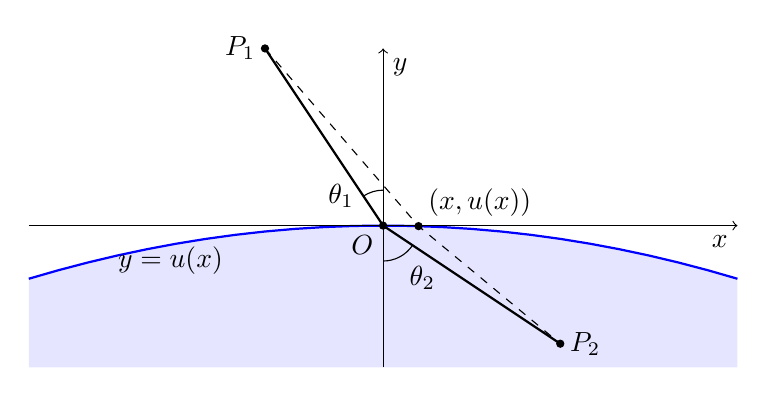
\begin{tikzpicture}[scale=1.5]
    % Surface (parabolic for illustration)
    \fill[blue!10] (-3,-1.2) -- (3,-1.2) -- plot[domain=3:-3] (\x, {-0.05*\x*\x}) -- cycle;
    \draw[thick, blue, domain=-3:3] plot (\x, {-0.05*\x*\x});
    \node at (-1.8,-0.3) { \( y = u(x) \) };

    % Axes
    \draw[->] (-3,0) -- (3,0) node[below left]{$x$};
    \draw[->] (0,-1.2) -- (0,1.5) node[below right]{$y$};
    
    
    % Point O
    \fill (0,0) circle (1pt) node[below left]{$O$};
    
    % Incident ray
    \draw[thick] (-1,1.5) -- (0,0);
    \fill (-1,1.5) circle (1pt) node[left]{$P_1$};
    
    % Refracted ray
    \draw[thick] (0,0) -- (1.5,-1);
    \fill (1.5,-1) circle (1pt) node[right]{$P_2$};
    
    % Variation ray
    \draw[dashed] (-1,1.5) -- (0.3,{-0.05*0.3*0.3}) -- (1.5,-1);
    \fill (0.3,{-0.05*0.3*0.3}) circle (1pt) node[above right]{$(x,u(x))$};

    % angles
    \draw (0,0.3) arc (90:123.69:0.3) node[left]{$\theta_1$};
    \draw (0,-0.3) arc (-90:-33.69:0.3) node[midway, below right]{$\theta_2$};
\end{tikzpicture}  \end{center}
\caption{Fermat's Principle, see exercise~\ref{ex:snell} on the derivation of Snell's Law.}
\end{figure}

It is hypothesized that between two sufficiently close points along the path of
the light ray, the light travels the path that minimizes the travel time.%
\footnote{
  This principle is known as Fermat's principle 
  and is the first formulation of the principle of least action in physics.
  In modern physics, the requirement of having a minimum is replaced with that 
  of having a stationary point.
  Thus, the thesis of Fermat's theorem is taken as the principle 
  instead of the hypothesis.
  }
It is also hypothesized that the speed of light is constant within each medium
(but different in the two media).

Consider the point $O$ where the light passes from one medium to another
and consider the plane containing the two incident and refracted rays at 
point $O$. On this plane, we place a Cartesian coordinate system 
with the $x$-axis oriented along the tangent plane at $O$ to the boundary 
surface between the two media and with the $y$-axis perpendicular 
to this surface. 
Let $(x_1,y_1)$ and $(x_2,y_2)$ be the coordinates of any two points $P_1$ and
$P_2$,
the first on the incident ray and the second on the refracted ray, different
from $O$
and sufficiently close to $O$ to hypothesize that the shortest path 
from $P_1$ to $P_2$ is the one that first traverses the segment 
from $P_1$ to $O$ and then the segment from $O$ to $P_2$.

The angle of incidence $\theta_1$ and the angle of refraction $\theta_2$
are thus given by the following formulas:
\[
  \sin \theta_1 = -\frac{x_1}{\sqrt{x_1^2+y_1^2}},\qquad
  \sin \theta_2 = \frac{x_2}{\sqrt{x_2^2+y_2^2}}.
\]

Let $u(x)$ be the function that describes the profile of the boundary 
surface between the two media. As we have chosen the coordinate system, we have
$u(0)=0$ and $u'(0)=0$.
%Suppose that $u$ is of class $C^1$.
We can then write the function $f(x)$ that represents
the travel time of a light ray that traverses 
the segment from $(x_1,y_1)$ to $(x,u(x))$ in the first medium and then 
the segment from $(x,u(x))$ to $(x_2,y_2)$ in the second medium.
If $c_1$ and $c_2$ are the speeds of light in the two media, 
we will have:
\[
  f(x) = \frac{1}{c_1} \sqrt{(x - x_1)^2 + (u(x) - y_1)^2} +
         \frac{1}{c_2} \sqrt{(x - x_2)^2 + (u(x) - y_2)^2}.
\]
By hypothesis, the function $f$ assumes a minimum at $x=0$, 
and thus, by Fermat's theorem, we must have $f'(0)=0$.
We then calculate the derivative of $f$ 
\[
    f'(x) = \frac{1}{c_1}\frac{x - x_1 + (u(x)-y_1)u'(x)}{\sqrt{(x-x_1)^2 +
  (u(x)-y_1)^2}} +
          \frac{1}{c_2}\frac{x - x_2 + (u(x)-y_2)u'(x)}{\sqrt{(x-x_2)^2 + (u(x)-y_2)^2}}
\]
and evaluate it at $x=0$, 
remembering that $u(0)=0$ and $u'(0)=0$:
\[
  f'(0) = \frac{1}{c_1}\frac{- x_1}{\sqrt{x_1^2 + y_1^2}} +
          \frac{1}{c_2}\frac{- x_2}{\sqrt{x_2^2 + y_2^2}}
        = \frac{\sin \theta_1}{c_1} - \frac{\sin \theta_2}{c_2}.
\]
The condition $f'(0)=0$ gives us Snell's Law:
\[
  \frac{\sin \theta_1}{c_1} = \frac{\sin \theta_2}{c_2}.
\]
\end{exercise}

\begin{theorem}[Rolle]
\mymark{***}
\index{theorem!of Rolle}
\mymargin{Rolle}%
\index{Rolle}
Let $f\colon [a,b]\to \RR$, $a,b\in \RR$, $a<b$, be a function continuous on the
entire $[a,b]$ and differentiable on $(a,b)$.
\mynote{If $b<a$, the theorem is equally valid 
if $[a,b]=[b,a]$ is understood}%
If $f(a) = f(b)$, then there exists $x_0 \in (a,b)$ such that $f'(x_0)=0$.
\end{theorem}
%
\begin{proof}
\mymark{***}
Since $f$ is a continuous function,
we can apply the Weierstrass theorem to deduce that $f$ has a maximum and 
minimum on the closed and bounded interval $[a,b]$. 
If the point of maximum or the point of minimum lies in the open interval 
$(a,b)$, we can apply Fermat's theorem to obtain that the derivative 
of $f$ vanishes at that point.

Otherwise, both the point of maximum and the point of minimum are endpoints 
of the interval, i.e., they are equal to $a$ or $b$. But since $f(a)=f(b)$, 
the maximum and minimum values coincide, and thus the function is constant. 
But in such a case, $f'(x)=0$ for every $x\in (a,b)$.
\end{proof}

\begin{theorem}[Lagrange]\label{th:lagrange}%
\mymark{***}%
\index{theorem!of Lagrange}%
\mymargin{Lagrange}%
\index{Lagrange}%
Let $f\colon [a,b]\to \RR$ be a function continuous on $[a,b]$ and
differentiable on $(a,b)$
with $a,b\in \RR$, $a<b$.
\mynote{If $b<a$, the theorem is equally valid 
if $[a,b]=[b,a]$ is understood}%
Then there exists a point $x_0\in (a,b)$ such that
\[
  f'(x_0) = \frac{f(b) - f(a)}{b-a}
\]
\end{theorem}
%
\begin{proof}
\mymark{***}
Consider the auxiliary function:
\[
  g(x) = f(x) - \frac{f(b)-f(a)}{b-a} x.
\]
By direct verification, we observe that
\[
  g(b) = g(a) = \frac{b f(a) - a f(b)}{b-a}.
\]
The function $g$ thus satisfies the hypotheses of Rolle's theorem, and therefore
there will exist $x_0\in (a,b)$ such that $g'(x_0)=0$.
But we observe that
\[
  g'(x) = f'(x) - \frac{f(b)-f(a)}{b-a}
\]
and thus if $g'(x_0)=0$, the desired result is obtained.
\end{proof}

\begin{theorem}[Monotonicity Criteria]%
\label{th:criteri_monotonia}
\mymark{***}%
\mymargin{monotonicity criteria}%
\index{criterion!of monotonicity}%
Let $f\colon I \to \RR$ be a function defined on an interval $I\subset \RR$. Let
$J= (\inf I, \sup I)$ be the open interval with the same endpoints as $I$.
Suppose that $f$ is continuous on $I$ and differentiable on $J$. 
Then the following criteria hold:
\begin{enumerate}
\item
$(\forall x \in J\colon f'(x)\ge 0)$
$\iff$
$f$ is non-decreasing (on the entire $I$);
\item
$(\forall x \in J\colon f'(x)\le 0)$
$\iff$
$f$ is non-increasing (on the entire $I$);
\item
$(\forall x \in J\colon f'(x)=0)$
$\iff$
$f$ is constant (on the entire $I$);
\item
$(\forall x \in J\colon f'(x)>0)$
$\implies$
$f$ is strictly increasing (on the entire $I$);
\item
$(\forall x \in J\colon f'(x)<0)$
$\implies$
$f$ is strictly decreasing (on the entire $I$).
\end{enumerate}
\end{theorem}
%
\begin{proof}
\mymark{***}
First, we prove the implications from left to right.

For the first, if $f$ were not non-decreasing, there would have to be two points
$a, b \in I$ such that $a < b$ but $f(a) > f(b)$.
Thus, we would have
\[
  \frac{f(b) - f(a)}{b - a} < 0.
\]
Applying Lagrange's theorem to the interval $[a,b]$, we would find a point $x\in
(a,b)$ such that $f'(x) < 0$. Clearly, $(a,b)\subset J$, and thus this
contradicts the hypothesis $f'(x) \ge 0$.

The second implication (for non-increasing functions) is proved similarly by
reversing the direction of the inequalities.

The third implication is proved using Lagrange's theorem in a manner similar to
the previous ones. Alternatively, it suffices to observe that if $f'(x)=0$, then
both $f'(x)\ge 0$ and $f'(x)\le 0$ hold simultaneously, so combining the first
two implications, we obtain that $f$ is both non-decreasing and non-increasing,
hence constant.

For the fourth implication, proceed as in the first. By contradiction, we would
have $a<b$ with $f(b) \le f(a)$. But then
\[
  \frac{f(b) - f(a)}{b-a} \le 0
\]
and applying Lagrange's theorem, we would find a point $x\in (a,b)$ with $f'(x)
\le 0$, against the hypothesis $f'(x) > 0$.

The fifth implication is proved similarly by reversing the direction of the
inequalities.

Now, let us consider the implications from right to left.
For the first, suppose that $f$ is non-decreasing and take $x\in J$. Then it is
clear that for every $h>0$, we will have $f(x+h) \ge f(x)$, and thus
\[
  \frac{f(x+h)- f(x)}{h} \ge 0.
\]
Taking the limit as $h \to 0^+$, we obtain $f'(x)$, and by the permanence of
sign, it must be $f'(x) \ge 0$.

Similarly (by reversing the inequalities), the second implication is proved.

The third follows from the first two or, more simply, from the rules of
differentiation, as the derivative of a constant is zero.
\end{proof}

\begin{example}
The function $f(x) = 1/x$ is defined on $\RR \setminus \ENCLOSE{0}$, is
differentiable,
and the derivative $f'(x) = -1/x^2$ is everywhere negative. The function $f$ is
thus strictly
decreasing separately on the two intervals $(0,+\infty)$ and $(-\infty,0)$ on
which
we can apply the monotonicity criterion. However, it is not
decreasing on its entire domain since, for example, $f(-1) = -1 < 1 = f(1)$.
This example shows that in the monotonicity criteria, the hypothesis that the
domain is an interval
is fundamental.
\end{example}

\begin{exercise}[Continuous Extension]
  \label{ex:estensione_continua_derivata_limitata}
Let $f\colon (a,b)\to \RR$ be a differentiable function with bounded derivative:
$\abs{f'(x)} \le L$ for every $x\in (a,b)$.
Then the limit of $f(x)$ as $x\to a^+$ and as $x\to b^-$ exists.
And if $f$ is also bounded, such limits are finite, thus 
$f$ extends continuously to the entire $[a,b]$.
\end{exercise}
\begin{proof}
If the limit of $f$ as $x\to a^+$ did not exist, then,
by the theorem~\ref{th:ponte} linking the limit of a function 
and the limit of a sequence, there would exist two sequences $a_n, b_n \to a^+$
such that $\lim f(a_n) \neq \lim f(b_n)$
(for example, $f(a_n)\to \limsup_{x\to a^+} f(x)$ and
$f(b_n)\to \liminf_{x\to a^+} f(x)$).
But by Lagrange's theorem, for each $n$, there would exist $c_n \in (a_n, b_n)$
such that
\[
  \abs{f'(c_n)} =
  \abs{\frac{f(b_n) - f(a_n)}{b_n - a_n}}
\]
and since $f(b_n)-f(a_n)$ does not tend to zero while $b_n - a_n \to 0$,
we would have $\abs{f'(c_n)} \to +\infty$,
contradicting the hypothesis that the derivative is bounded.
Thus, the limit of $f$ as $x\to a^+$ exists, and similarly, it is shown that the
limit
of $f$ as $x\to b^-$ exists.

If furthermore $f$ is bounded,
then the limits found are finite, and 
thus $f$ extends continuously to a function $\tilde f\colon [a,b]\to \RR$ 
defined as
\[
  \tilde f(x) = \begin{cases}
    f(x) & \text{if }x\in (a,b),\\
    \displaystyle\lim_{x\to a^+} f(x) & \text{if } x=a,\\
    \displaystyle\lim_{x\to b^-} f(x) & \text{if } x=b.
  \end{cases}
\]
\end{proof}